\documentclass[aps,prd,twocolumn,nofootinbib,superscriptaddress,10pt]{revtex4-2}

\usepackage{amsmath,amssymb,bm}
\usepackage{graphicx}
\usepackage{booktabs}
\usepackage{dcolumn}
\usepackage[colorlinks=true,linkcolor=blue,citecolor=blue,urlcolor=blue]{hyperref}

\newcommand{\ii}{\mathrm{i}}
\newcommand{\dd}{\mathrm{d}}
\newcommand{\rp}{r_+}
\newcommand{\rminus}{r_-}
\newcommand{\OmH}{\Omega_H}
\newcommand{\Bin}{B^{\rm inc}}
\newcommand{\Bref}{B^{\rm ref}}
\newcommand{\Btrans}{B^{\rm trans}}
\newcommand{\calO}{\mathcal{O}}

\begin{document}

\title{Endpoint-collocation spectral amplitudes for scalar Teukolsky scattering on Kerr}

\author{KerrScattering Project}
\affiliation{Manuscript draft generated from the KerrScattering repository}

\date{\today}

\begin{abstract}
We present a direct Chebyshev spectral construction of scalar
($s=0$) Teukolsky scattering amplitudes on a Kerr black hole.  The method is
designed as the Kerr continuation of a Schwarzschild Green-function spectral
code: the compact coordinate is $z=\rp/r$, the physical endpoints $z=0$ and
$z=1$ are retained as collocation nodes, and the degeneracy of the second-order
radial equation at both endpoints is used as a regular first-order boundary
condition.  With the horizon normalization $\Btrans=1$, the incident and
reflected amplitudes are obtained by matching a horizon-normalized in solution
to down/up solutions at an intermediate radius.  The invariant validation
quantities are $|\Bin|$, $|\Bref|$, and the Kerr flux balance relation; complex
phases are convention dependent because of the additive constant in the Kerr
tortoise coordinate.  Across 37 independent GeneralizedSasakiNakamura.jl
benchmark cases, including nonrotating, moderate-spin, near-superradiant, and
high-spin configurations, the worst amplitude-magnitude discrepancy is
$1.485\times 10^{-8}$ and the worst flux residual is
$3.714\times 10^{-9}$.  A 51-point frequency sweep resolves scalar
superradiance, with amplification appearing only for
$\omega<m\Omega_H$.  We also describe the implemented spheroidal cubic
projector and a first Green-function radial diagnostic for weak
$|\Phi|^2\Phi$ sources.  The latter is a diagnostic framework rather than a
final nonlinear Kerr normalization, and it identifies the remaining task:
deriving the covariant Kerr radial source weight and replacing finite
diagnostic quadrature by controlled oscillatory-tail integration.
\end{abstract}

\maketitle

\section{Introduction}

The Teukolsky formalism separates massless field perturbations on a Kerr black
hole into angular spheroidal harmonics and a radial ordinary differential
equation~\cite{Teukolsky1973}.  For scalar fields the system is already rich
enough to test the central numerical issues that appear in Kerr scattering:
horizon phase normalization, superradiant flux balance, spheroidal angular
mixing, and the conditioning of small reflected amplitudes.  The purpose of
this work is not to introduce a new radial equation, but to make the numerical
continuation from a Schwarzschild spectral Green-function code to Kerr precise
and reproducible.

The central design choice is to keep the physical boundaries in the collocation
grid.  In the compact coordinate $z=\rp/r$, infinity is at $z=0$ and the event
horizon is at $z=1$.  After peeling off the known oscillatory asymptotic
factor, the radial equation becomes singularly regular: the coefficient of the
second derivative vanishes at each endpoint, leaving a first-order condition.
This mirrors the endpoint treatment in the Schwarzschild spectral method and
avoids artificial horizon or infinity truncation.

The implementation is validated against GeneralizedSasakiNakamura.jl in the
unit-Teukolsky-transmission convention.  We use only invariant quantities for
the pass/fail comparison: amplitude magnitudes and the flux balance residual.
The complex amplitudes themselves are not invariant under a shift
$r_*\rightarrow r_*+C$ and therefore differ by constant phases across packages.

The remainder of this paper is organized as follows.  Section~\ref{sec:eqs}
sets the scalar Teukolsky conventions.  Section~\ref{sec:spectral} describes
the endpoint spectral discretization and amplitude extraction.
Section~\ref{sec:validation} gives the benchmark and frequency-sweep results.
Section~\ref{sec:nonlinear} describes the cubic spheroidal projector and the
current nonlinear Green-function diagnostic.  Section~\ref{sec:spinminus2}
summarizes the separate $s=-2$ benchmark side task.  We conclude in
Sec.~\ref{sec:conclusion}.

\section{Scalar Teukolsky equation on Kerr}
\label{sec:eqs}

\subsection{Geometry and tortoise coordinate}

In Boyer--Lindquist coordinates,
\begin{align}
\Sigma &= r^2+a^2\cos^2\theta,\\
\Delta &= r^2-2Mr+a^2=(r-\rp)(r-\rminus),\\
\rp &= M+\sqrt{M^2-a^2},\qquad
\rminus = M-\sqrt{M^2-a^2}.
\end{align}
The horizon angular velocity is
\begin{equation}
\OmH=\frac{a}{\rp^2+a^2}=\frac{a}{2M\rp}.
\end{equation}
We use the Kerr tortoise coordinate
\begin{equation}
\frac{\dd r_*}{\dd r}=\frac{r^2+a^2}{\Delta},
\end{equation}
so that
\begin{equation}
r_*=r+\frac{2M\rp}{\rp-\rminus}\ln(r-\rp)
       -\frac{2M\rminus}{\rp-\rminus}\ln(r-\rminus)+C.
\end{equation}
The constant $C$ fixes a phase convention but has no invariant content.

\subsection{Angular equation and separation constant}

For a massless complex scalar field, $\Box\Phi=0$, we separate
\begin{equation}
\Phi(t,r,\theta,\phi)=
R_{\ell m\omega}(r)S_{\ell m}(\theta;a\omega)
e^{\ii m\phi-\ii\omega t}.
\end{equation}
The scalar spheroidal function satisfies
\begin{align}
0={}&
\frac{1}{\sin\theta}\frac{\dd}{\dd\theta}
\left(\sin\theta\frac{\dd S_{\ell m}}{\dd\theta}\right)
\notag\\
&+
\left[
a^2\omega^2\cos^2\theta
-\frac{m^2}{\sin^2\theta}
 + A_{\ell m}
\right]S_{\ell m}.
\end{align}
For $c=a\omega\rightarrow0$, $A_{\ell m}\rightarrow \ell(\ell+1)$ and
$S_{\ell m}$ reduces to the corresponding spherical harmonic with the
$e^{\ii m\phi}$ factor removed.  The radial separation constant used here is
\begin{equation}
\lambda=A_{\ell m}+a^2\omega^2-2am\omega.
\label{eq:lambda}
\end{equation}
This convention is recorded explicitly in the output files, because different
packages return either $A_{\ell m}$ or a radial separation constant.

\subsection{Radial equation and asymptotics}

Defining
\begin{equation}
K(r)=(r^2+a^2)\omega-am,
\end{equation}
the scalar radial Teukolsky equation is
\begin{equation}
\frac{\dd}{\dd r}\left(\Delta\frac{\dd R}{\dd r}\right)
+\left(\frac{K^2}{\Delta}-\lambda\right)R=0 .
\label{eq:radial}
\end{equation}
Near the horizon the physical frequency is
\begin{equation}
p=\omega-m\OmH .
\end{equation}
The in solution is normalized by
\begin{equation}
R_{\rm in}\sim \Btrans e^{-\ii p r_*},\qquad \Btrans=1,
\qquad r\rightarrow \rp .
\label{eq:horizon_norm}
\end{equation}
At infinity,
\begin{equation}
R_{\rm in}\sim
\Bin \frac{e^{-\ii\omega r_*}}{r}
+\Bref \frac{e^{+\ii\omega r_*}}{r}.
\label{eq:infinity_amp}
\end{equation}
The up solution is purely outgoing at infinity,
\begin{equation}
R_{\rm up}\sim \frac{e^{+\ii\omega r_*}}{r}.
\end{equation}

\subsection{Wronskian and flux}

Equation~\eqref{eq:radial} has a conserved radial Wronskian
\begin{equation}
W[R_1,R_2]=\Delta\left(R_1\frac{\dd R_2}{\dd r}
-R_2\frac{\dd R_1}{\dd r}\right).
\end{equation}
For the normalization \eqref{eq:horizon_norm}, the scalar flux relation is
\begin{equation}
\mathcal R+\mathcal T=1,
\end{equation}
with
\begin{equation}
\mathcal R=\frac{|\Bref|^2}{|\Bin|^2},\qquad
\mathcal T=
\frac{p(\rp^2+a^2)}{\omega}
\frac{|\Btrans|^2}{|\Bin|^2}.
\label{eq:flux}
\end{equation}
For $\omega<m\OmH$, $\mathcal T<0$ and therefore $\mathcal R>1$, which is the
scalar superradiant regime~\cite{PressTeukolsky1972}.

\section{Endpoint Chebyshev spectral construction}
\label{sec:spectral}

\subsection{Compactification and phase peeling}

We use
\begin{equation}
z=\frac{\rp}{r},\qquad z=0\ {\rm at}\ \mathcal{I}^+,\qquad z=1\ {\rm at}\ H^+ .
\end{equation}
Each homogeneous branch is written as
\begin{equation}
R(z)=F_{\rm branch}(z)u(z),
\end{equation}
where $F_{\rm branch}$ contains the known asymptotic phase:
\begin{align}
F_{\rm down} &= e^{-\ii\omega r_*}/r,\\
F_{\rm up} &= e^{+\ii\omega r_*}/r,\\
F_{\rm in} &= e^{-\ii p r_*}.
\end{align}
The reduced function $u(z)$ is smooth at the relevant endpoint and is
normalized by $u=1$ there.

After substitution, each branch has the schematic equation
\begin{equation}
B_2(z)u''+B_1(z)u'+B_0(z)u=0.
\label{eq:peeled}
\end{equation}
At $z=0$ and $z=1$, $B_2$ vanishes.  The collocation matrix therefore keeps the
degenerate endpoint row as a first-order regularity condition and uses the
neighboring row to impose $u({\rm endpoint})=1$.  No finite-radius horizon or
infinity cutoff is introduced.

\subsection{Two-domain matching}

The implementation uses two Chebyshev domains, $[0,z_m]$ and $[z_m,1]$.
On the outer domain we solve the down and up branches.  On the inner domain we
solve the horizon-normalized in branch.  At $z_m=\rp/r_m$ the physical field
and radial derivative satisfy
\begin{equation}
R_{\rm in}= \Bin R_{\rm down}+\Bref R_{\rm up},
\end{equation}
\begin{equation}
\frac{\dd R_{\rm in}}{\dd r}=
\Bin \frac{\dd R_{\rm down}}{\dd r}
+\Bref \frac{\dd R_{\rm up}}{\dd r}.
\end{equation}
Thus $\Bin$ and $\Bref$ are obtained from a $2\times2$ linear system.  The
matching radius and spectral order are selected adaptively in the validation
scripts, with sinh clustering used for low-frequency cases when useful.

\section{Linear validation}
\label{sec:validation}

\subsection{GSN benchmark protocol}

The external benchmark is GeneralizedSasakiNakamura.jl~\cite{GSN} in the
\texttt{UNIT\_TEUKOLSKY\_TRANS} convention.  We compare
$|\Bin|$, $|\Bref|$, and the flux residual.  The complex phases are retained in
CSV output but not used as benchmark errors, because a shift in $r_*$ maps
\begin{equation}
\Bin\rightarrow \Bin e^{-\ii\omega C},\qquad
\Bref\rightarrow \Bref e^{+\ii\omega C}.
\end{equation}

The acceptance gates are
\begin{align}
\frac{\delta|\Bin|}{|\Bin|}&\leq 10^{-7},&
\frac{\delta|\Bref|}{|\Bref|}&\leq 10^{-7},\notag\\
|\mathcal R+\mathcal T-1|&\leq 10^{-8}.
\end{align}

\begin{table}[t]
\caption{Validation summary for the scalar Kerr spectral solver.  The
``score'' is the maximum of the invariant amplitude-magnitude errors and the
flux residual.}
\label{tab:summary}
\begin{ruledtabular}
\begin{tabular}{lc}
Quantity & Value\\
\hline
GSN benchmark requests & 37\\
Usable GSN cases & 37\\
Excluded GSN cases & 0\\
All GSN cases passed & true\\
Worst score & $1.485\times10^{-8}$\\
Worst flux residual & $3.714\times10^{-9}$\\
Frequency-sweep points & 51\\
Worst sweep score & $9.467\times10^{-8}$\\
Worst sweep flux residual & $7.351\times10^{-9}$\\
Maximum sampled $\mathcal R-1$ & $4.970\times10^{-4}$\\
\end{tabular}
\end{ruledtabular}
\end{table}

The benchmark grid covers the Schwarzschild limit, moderate Kerr rotation,
near-threshold scalar superradiance, low-frequency superradiant scattering,
high-frequency small-reflection scattering, and high-spin cases.  The hardest
case is $(a,\ell,m,\omega)=(0.5,2,2,1.0)$, where the reflected amplitude is
small and the relative error is correspondingly sensitive to conditioning.

\begin{figure}[t]
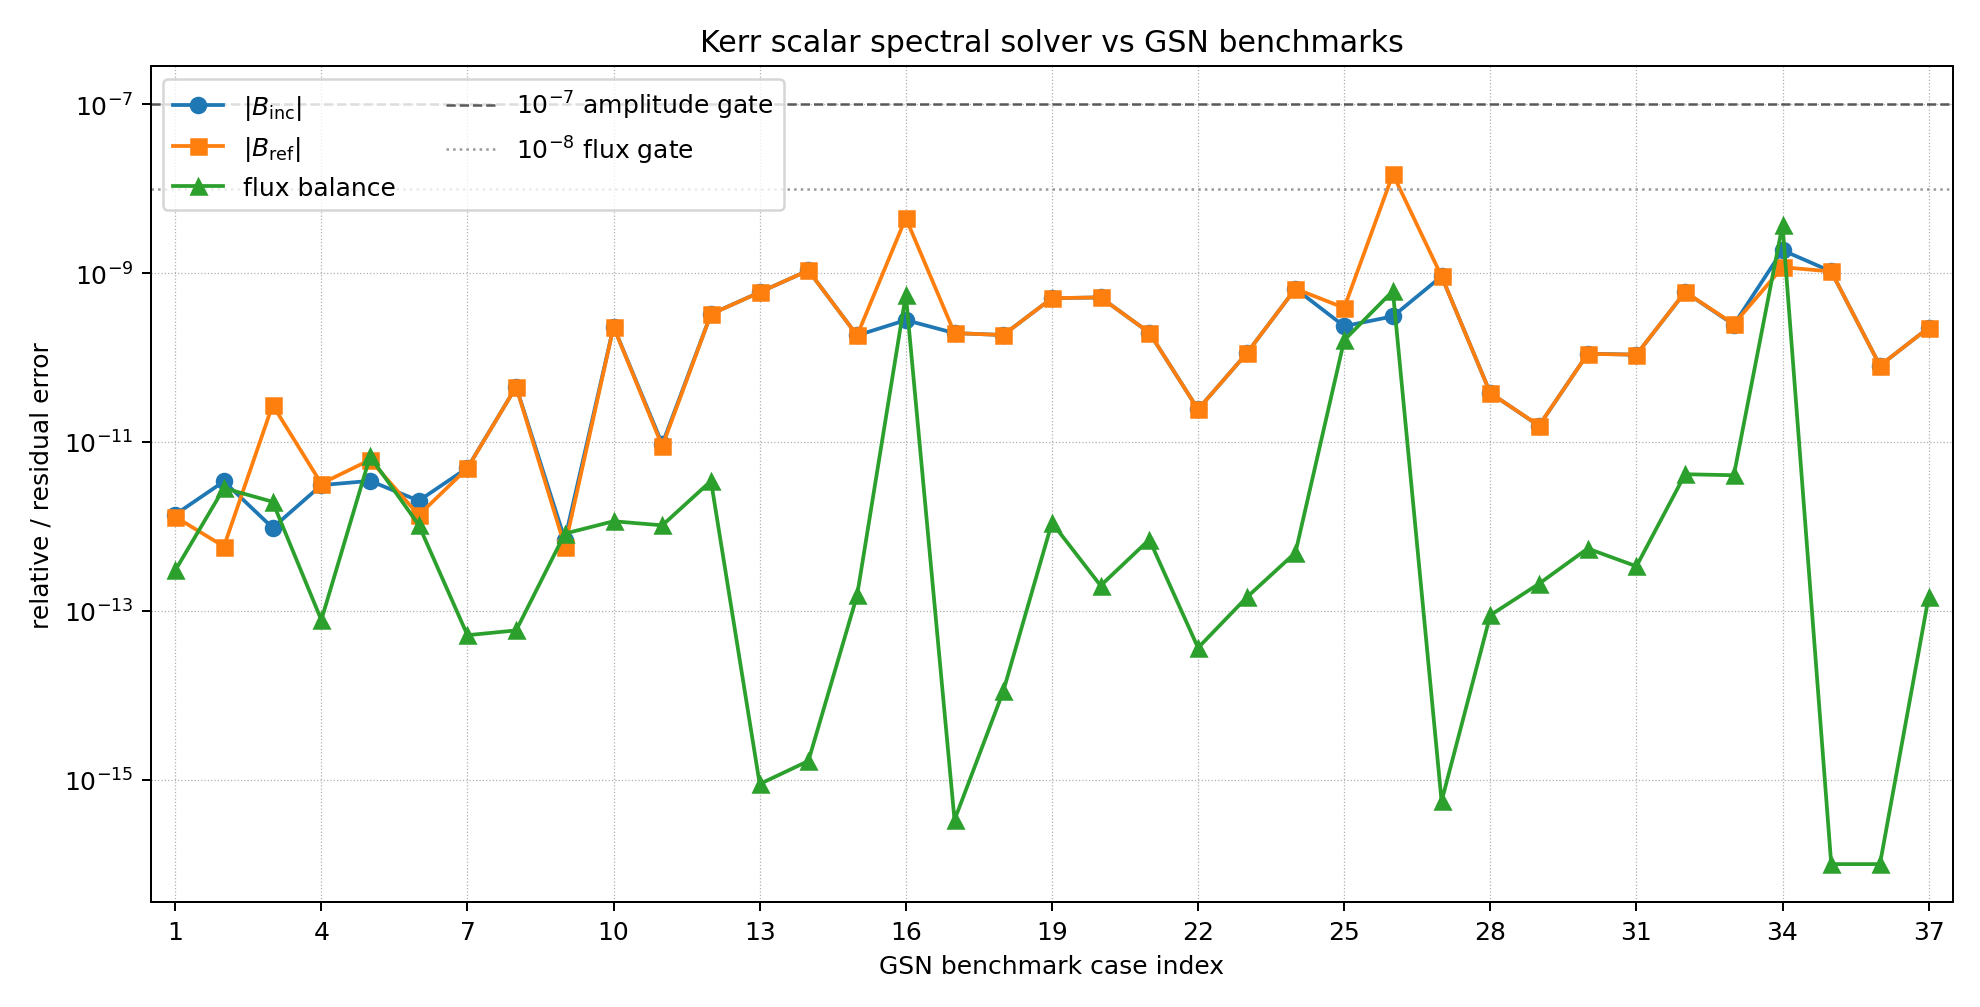
\includegraphics[width=\columnwidth]{../../figures/kerr_scalar_adaptive_errors.png}
\caption{Invariant GSN benchmark errors for the validated scalar Kerr grid.
Only amplitude magnitudes and flux balance are used for pass/fail decisions.}
\label{fig:benchmark_errors}
\end{figure}

\subsection{Frequency sweep and superradiance}

The frequency sweep contains one Schwarzschild reference sequence and two Kerr
sequences:
\begin{align}
&a=0,\quad \ell=m=0,\quad 11\ {\rm points},\\
&a=0.5,\quad \ell=m=2,\quad 20\ {\rm points},\\
&a=0.9,\quad \ell=m=2,\quad 20\ {\rm points}.
\end{align}
For the rotating cases the sampled amplification $\mathcal R-1$ is positive
only for $\omega<m\OmH$, in agreement with Eq.~\eqref{eq:flux}.

\begin{figure}[t]
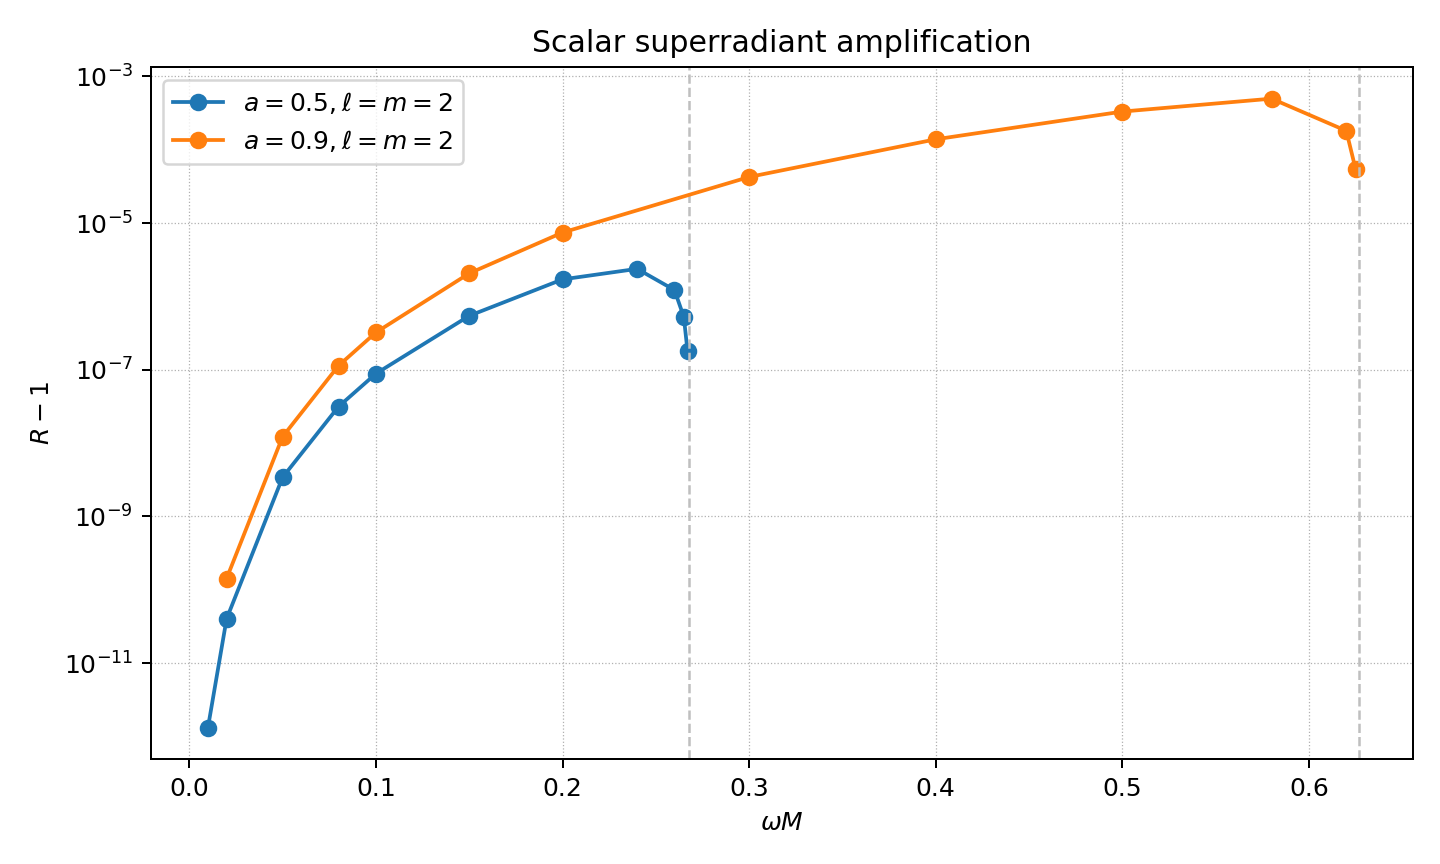
\includegraphics[width=\columnwidth]{../../figures/kerr_scalar_superradiance_amplification.png}
\caption{Sampled scalar superradiant amplification.  Positive amplification is
confined to the region $\omega<m\Omega_H$.}
\label{fig:superradiance}
\end{figure}

\section{Cubic angular projector and nonlinear diagnostic}
\label{sec:nonlinear}

For a weak complex scalar self-interaction,
\begin{equation}
\Box\Phi+\epsilon |\Phi|^2\Phi=0,
\end{equation}
a single incident mode sources the angular structure
$|S_{\ell m}|^2S_{\ell m}$.  This must be projected onto the spheroidal basis:
\begin{equation}
|S_{\ell m}|^2S_{\ell m}
=\sum_{\ell'} C_{\ell'\ell m} S_{\ell' m},
\end{equation}
where
\begin{equation}
C_{\ell'\ell m}
=\int \dd\Omega\,
S^*_{\ell' m}|S_{\ell m}|^2S_{\ell m}.
\label{eq:cubic}
\end{equation}
The code evaluates Eq.~\eqref{eq:cubic} for every validated source mode and
target channels $|m|\leq \ell'\leq \ell+4$.  The present table contains
199 coupling rows from 37 source modes.  The self-channel coefficient ranges
from $7.958\times10^{-2}$ to $1.705\times10^{-1}$, while the largest
off-diagonal coefficient is $8.318\times10^{-2}$ for
$(\ell,m,a,\omega,\ell')=(2,0,0.5,0.1,4)$.  The spherical checks
$C_{000}=1/(4\pi)$ and $C_{110}=9/(20\pi)$ are satisfied.

The nonlinear radial diagnostic uses the validated homogeneous solutions and
the conserved Wronskian to compute prototype Green-function source integrals.
At present the radial source weight is explicitly labelled
\texttt{legacy-bondi-dr-over-r2}; it is a diagnostic bridge from the
Schwarzschild code, not a final Kerr self-interaction convention.  With four
representative cases and quadrature orders $64,96,128,192$, the worst
Wronskian consistency error is $3.094\times10^{-16}$.  The worst consecutive
quadrature changes are $7.011\times10^{-5}$ for the reflected correction and
$8.331\times10^{-5}$ for the horizon correction.  The run is resource guarded;
the recorded peak process RSS for the current diagnostic table is 83.0 MB.

\begin{table}[t]
\caption{Prototype nonlinear Green-function diagnostic amplitudes at
quadrature order $q=192$.  The amplitudes use the diagnostic
\texttt{legacy-bondi-dr-over-r2} radial weight and should not yet be read as
final Kerr nonlinear scattering observables.  Full complex values are stored in
\texttt{results/kerr\_scalar\_nonlinear\_diagnostics.csv}.}
\label{tab:nonlinear_diag}
\scriptsize
\begin{ruledtabular}
\begin{tabular}{lcccc}
case & $(a,\omega)$ &
$|A_{\rm ref}^{(1)}|$ & $|A_{H}^{(1)}|$ &
$\max\delta A$\\
\hline
Schw. $(0,0)$ & $(0,0.10)$ & $2.808\times10^{-2}$ &
$1.704\times10^{-2}$ & $2.103\times10^{-5}$\\
Kerr sub. & $(0.5,0.24)$ & $7.780\times10^{2}$ &
$1.836$ & $5.083\times10^{-7}$\\
Kerr super. & $(0.5,0.30)$ & $1.197\times10^{2}$ &
$7.645\times10^{-1}$ & $9.627\times10^{-7}$\\
High spin & $(0.9,0.58)$ & $1.298\times10^{1}$ &
$5.683\times10^{-1}$ & $3.164\times10^{-6}$\\
\end{tabular}
\end{ruledtabular}
\end{table}

These diagnostics show that the homogeneous Green-function skeleton is stable.
The remaining nonlinear physics is the derivation of the Kerr covariant radial
source weight and the replacement of finite diagnostic quadrature by an
oscillatory-tail method with explicit convergence gates.

\section{Spin-minus-two benchmark side task}
\label{sec:spinminus2}

The repository also records a separate $s=-2$ benchmark task for
$a=0.5$, $\ell=m=2$, and $\omega=10^{-4},0.1,10$.  Low and intermediate
frequencies are compared against a Mathematica MST route~\cite{ManoSuzukiTakasugi1996},
while the high frequency case uses GeneralizedSasakiNakamura.jl.  The direct
Teukolsky-variable Python comparison gives relative errors
\begin{align}
\omega=10^{-4}:&\quad
\delta \Bin/\Bin=2.5\times10^{-8},
\notag\\
&\quad
\delta \Bref/\Bref=9.1\times10^{-12},\\
\omega=0.1:&\quad
\delta \Bin/\Bin=2.7\times10^{-10},
\notag\\
&\quad
\delta \Bref/\Bref=5.3\times10^{-12},\\
\omega=10:&\quad
\delta \Bin/\Bin=4.0\times10^{-7},
\notag\\
&\quad
\delta \Bref/\Bref=3.4\times10^{-1}.
\end{align}
The high-frequency reflected amplitude is approximately $10^{-8}$, close to
the double-precision floor for direct Teukolsky-variable matching.  Pushing that
case to benchmark accuracy should be done in the Sasaki--Nakamura
variable~\cite{SasakiNakamura1982}, followed by the Teukolsky conversion.  This
side task is therefore kept separate from the scalar solver.

\section{Conclusions}
\label{sec:conclusion}

We have constructed and validated a Kerr scalar scattering solver that follows
the same endpoint-collocation philosophy as the Schwarzschild spectral
Green-function code.  The key points are: the compact coordinate $z=\rp/r$
keeps both physical boundaries in the grid; phase peeling converts the endpoint
singularities into regular first-order rows; horizon-normalized in modes are
matched to down/up modes to extract $\Bin$ and $\Bref$; and the invariant flux
balance provides a stringent convention-independent check.

The linear scalar problem is closed at the level required for a publication
draft: 37 GSN benchmark cases and 51 frequency-sweep points pass the stated
acceptance gates, and the sweep resolves the expected Kerr superradiant
amplification.  The cubic angular projector and first radial Green-function
diagnostics are implemented, but the nonlinear source normalization is not yet
final.  The next physics step is to derive the Kerr radial source weight from
the covariant scalar equation and to introduce a controlled oscillatory-tail
integration method for nonlinear amplitudes.

\begin{acknowledgments}
This draft was generated from the numerical outputs in the KerrScattering
repository on the branch \texttt{codex/teukolsky-scalar-derivation}.  The
external scalar benchmark uses GeneralizedSasakiNakamura.jl.
\end{acknowledgments}

\section*{Data and code availability}

The validation data are stored in CSV files under \texttt{results/}.  The main
files used in this manuscript are
\texttt{kerr\_scalar\_adaptive\_summary.csv},
\texttt{kerr\_scalar\_frequency\_sweep.csv},
\texttt{kerr\_scalar\_cubic\_couplings.csv}, and
\texttt{kerr\_scalar\_nonlinear\_diagnostics.csv}.

\begin{thebibliography}{9}

\bibitem{Teukolsky1973}
S. A. Teukolsky,
Perturbations of a rotating black hole. I. Fundamental equations for
gravitational, electromagnetic, and neutrino-field perturbations,
Astrophys. J. \textbf{185}, 635 (1973).

\bibitem{PressTeukolsky1972}
W. H. Press and S. A. Teukolsky,
Floating orbits, superradiant scattering and the black-hole bomb,
Nature \textbf{238}, 211 (1972).

\bibitem{SasakiNakamura1982}
M. Sasaki and T. Nakamura,
A class of new perturbation equations for the Kerr geometry,
Prog. Theor. Phys. \textbf{67}, 1788 (1982).

\bibitem{ManoSuzukiTakasugi1996}
S. Mano, H. Suzuki, and E. Takasugi,
Analytic solutions of the Teukolsky equation and their low frequency
expansions,
Prog. Theor. Phys. \textbf{95}, 1079 (1996).

\bibitem{GSN}
R. K. L. Lo,
GeneralizedSasakiNakamura.jl,
\url{https://github.com/ricokaloklo/GeneralizedSasakiNakamura.jl}.

\end{thebibliography}

\end{document}
